\documentclass[varwidth,border=10pt]{standalone}

\usepackage[aboveskip=1pt,labelfont=bf,labelsep=period,justification=raggedright,singlelinecheck=off]{caption}
\usepackage{amsmath}
\usepackage{tikz}
\usepackage{tikz-cd}
\usetikzlibrary{matrix,arrows,positioning,calc,shapes,arrows.meta}
\usepackage{xstring}
\tikzset{  
	-Latex,auto,node distance =1.5 cm and 1.3 cm, thick,% node distance is the distance between one node to other, where 1.5cm is the length of the edge between the nodes  
	state/.style ={ellipse, draw, minimum width = 0.9 cm}, % the minimum width is the width of the ellipse, which is the size of the shape of vertex in the node graph  
	point/.style = {circle, draw, inner sep=0.18cm, fill, node contents={}},  
	bidirected/.style={Latex-Latex,dashed}, % it is the edge having two directions  
	el/.style = {inner sep=2.5pt, align=right, sloped}  
} 
%\usepackage[subrefformat=parens, labelfont=up]{subcaption}
%\usepackage{cleveref}
%\crefname{thm}{Theorem}{Theorems}
\setlength{\textwidth}{\dimexpr 6in\relax}
\usepackage{makecell}



\newcommand{\bbB}{\mathbb{B}}
\newcommand{\bL}{\mathbb{L}}
\newcommand{\bU}{\mathbb{U}}

\newcommand{\cL}{\mathcal{L}}
\newcommand{\cM}{\mathcal{M}}

\newcommand{\Targets}{\mathbf{T}}
\newcommand{\Sources}{\mathbf{S}}

\newcounter{countitems}


\newcommand{\boolf}{{\mathfrak 0}}
\newcommand{\boolt}{{\mathfrak 1}}

\newcommand{\bzero}{{\bf 0}}
\newcommand{\bone}{{\bf 1}}

\newcommand{\setof}[1]{\left\{ {#1}\right\}}
\newcommand{\setdef}[2]{\left\{{#1}\,\left|\,{#2}\right.\right\}}

\usepackage[subrefformat=parens, labelfont=up]{subcaption}

\begin{document}

\begin{figure}[h!]
    \centering
    \begin{subfigure}{0.49\textwidth}
        \centering
        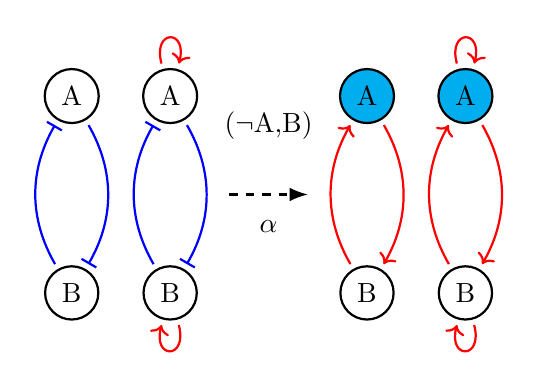
\begin{tikzpicture}[every node/.style={circle,fill=white!20,thick,draw},scale=2.5,
        blueedge/.style={thick,blue,-|,shorten <=2pt,shorten >=2pt},
        rededge/.style={thick,red,->,shorten <=2pt,shorten >=2pt},
        textbox/.style={draw=none, fill=none, midway}
        ]
            \node (A) at (0,1) {A};
            \node (B) at (0,0) {B};
            \node (ASA) at (0.5,1) {A};
            \node (BSA) at (0.5,0) {B};
            \node[fill=cyan] (AP) at (1.5,1) {A};
            \node (BP) at (1.5,0) {B};
            \node[fill=cyan] (APSA) at (2,1) {A};
            \node (BPSA) at (2,0) {B};
            \path[blueedge, bend left] 
                (A) edge (B)
                (B) edge (A)
                (ASA) edge (BSA)
                (BSA) edge (ASA);
            \path[rededge, bend left] 
                (AP) edge (BP)
                (BP) edge (AP)
                (APSA) edge (BPSA)
                (BPSA) edge (APSA);
            \path[rededge, loop above, min distance=6pt]
                (ASA) edge (ASA)
                (APSA) edge (APSA);
            \path[rededge, loop below, min distance=6pt]
                (BSA) edge (BSA)
                (BPSA) edge (BPSA);
            \draw[dashed, thick] (0.8,0.5) -- (1.2,0.5) 
                node[textbox, above=1.2mm] {($\neg$A,B)}
                node[textbox, below=1mm] {$\alpha$};
        \end{tikzpicture}
    \caption{}
    \label{fig:TS}
    \end{subfigure}
    \begin{subfigure}{0.49\textwidth}
        \centering
        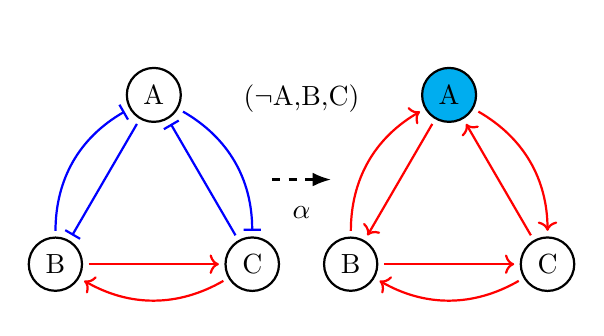
\begin{tikzpicture}[scale=2.5,
            every node/.style={circle,fill=white!20,thick,draw},
            blueedge/.style={thick,blue,-|,shorten <=2pt,shorten >=2pt},
            rededge/.style={thick,red,->,shorten <=2pt,shorten >=2pt},
            textbox/.style={draw=none, fill=none, midway}
        ]
            \node (A) at (0.5,0.86) {A};
            \node (B) at (0,0) {B};
            \node (C) at (1,0) {C};
            \node[fill=cyan] (AP) at (2,0.86) {A};
            \node (BP) at (1.5,0) {B};
            \node (CP) at (2.5,0) {C};
            \path[blueedge] 
                (A) edge (B)
                (B) edge[bend left] (A)
                (A) edge[bend left] (C)
                (C) edge (A);
            \path[rededge]
                (B) edge (C)
                (C) edge[bend left] (B)
                (AP) edge (BP)
                (BP) edge[bend left] (AP)
                (AP) edge[bend left] (CP)
                (CP) edge (AP)
                (BP) edge (CP)
                (CP) edge[bend left] (BP);
            \draw[dashed, thick] 
                (1.1,0.43) -- (1.4,0.43)
                node[textbox, above=1.2mm] {($\neg$A,B,C)}
                node[textbox, below=1mm] {$\alpha$};
        \end{tikzpicture}
    \caption{}
    \label{fig:3Team}
    \end{subfigure}
    
    \begin{subfigure}{0.6\textwidth}
        \centering
        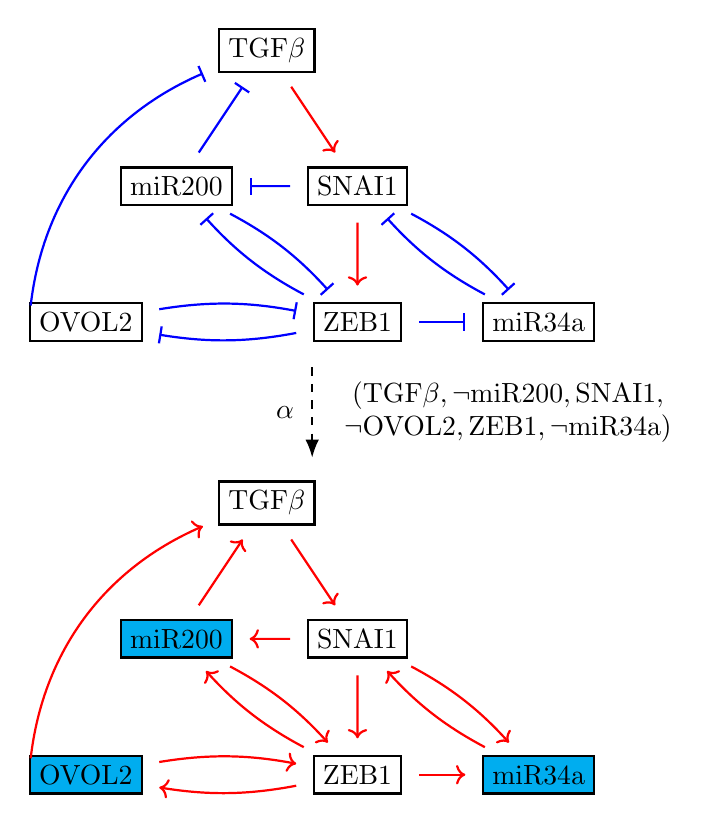
\begin{tikzpicture}[scale=2.3,
            every node/.style={rectangle,fill=white!20,thick,draw},
            blueedge/.style={thick,blue,-|,shorten <=6pt,shorten >=6pt},
            rededge/.style={thick,red,->,shorten <=6pt,shorten >=6pt},
            textbox/.style={draw=none, fill=none, midway}
        ]
            \node (tgb) at (1,1.5) {TGF$\beta$};
            \node (m200) at (0.5,0.75) {miR200};
            \node (snl) at (1.5,0.75) {SNAI1};
            \node (ovl) at (0,0) {OVOL2};
            \node (zeb) at (1.5,0) {ZEB1};
            \node (m34) at (2.5,0) {miR34a};
            \path[blueedge, bend left=10] 
                (zeb) edge (ovl)
                (ovl) edge (zeb)
                (m200) edge (zeb)
                (zeb) edge (m200)
                (snl) edge (m34)
                (m34) edge (snl);
            \path[blueedge] 
                (ovl.west) edge[bend left] (tgb);
            \path[blueedge]
                (m200) edge (tgb)
                (zeb) edge (m34)
                (snl) edge (m200);
            \path[rededge]
                (tgb) edge (snl)
                (snl) edge (zeb);
            \begin{scope}[yshift=-2.5cm]
            \node (tgb2) at (1,1.5) {TGF$\beta$};
            \node [fill=cyan] (m200_2) at (0.5,0.75) {miR200};
            \node (snl2) at (1.5,0.75) {SNAI1};
            \node [fill=cyan] (ovl2) at (0,0) {OVOL2};
            \node (zeb2) at (1.5,0) {ZEB1};
            \node [fill=cyan] (m34_2) at (2.5,0) {miR34a};
            \path[rededge, bend left=10] 
                (zeb2) edge (ovl2)
                (ovl2) edge (zeb2)
                (m200_2) edge (zeb2)
                (zeb2) edge (m200_2)
                (snl2) edge (m34_2)
                (m34_2) edge (snl2);
            \path[rededge] 
                (ovl2.west) edge[bend left] (tgb2);
            \path[rededge]
                (m200_2) edge (tgb2)
                (zeb2) edge (m34_2)
                (snl2) edge (m200_2)
                (tgb2) edge (snl2)
                (snl2) edge (zeb2);
            \end{scope}
            \draw[dashed, thick] (1.25,-0.25) -- (1.25,-0.75) 
                node[textbox, right=1mm] {$\begin{array}{c}
                    (\text{TGF}\beta, \neg\text{miR200}, \text{SNAI1},\\
                    \neg\text{OVOL2}, \text{ZEB1}, \neg\text{miR34a})
                    \end{array}$}
                node[textbox, left=1mm] {$\alpha$};
        \end{tikzpicture}
    \caption{}
    \label{fig:EMT6N}
    \end{subfigure}
    \label{fig:changevar}
\end{figure}

\end{document}